\chapter{Численные эксперименты}
\label{chapter:experiments} \index{Эксперименты}

В данной главе приведены результаты численных экспериментов,
целью которых является проверка работы предложенных методов
на примере жёстких систем дифференциальных уравнений.
Невязка и матрица Якоби вычисляются при помощи систем автодифференцирования.
Решение систем линейных алгебраических уравнений производится при помощи библиотеки INMOST \cite{vassilevski2020parallel}.
Диагонализация матрицы производится при помощи библиотеки Eigen \cite{eigenweb}.
В этой секции референсным решением будет называться численное решение,
полученное методом трапеций при использовании малого шага по времени ($ 10^5 $ точек).
Допустимая погрешность в методе Ньютона: $ \abseps = 10^{-7} $ и $ \releps = 10^{-9} $.
Максимальное допустимое число ньютоновских итераций: $ N = 200 $.



\section{Система Лотки-Вольтерры}
\label{sec:Lotka-Volterra}

Система Лотки-Вольтерры \cite{lotka1925elements} имеет вид
%
\begin{equation}
    \label{eq:Lotka-Volterra_system}
    \begin{dcases}
        \frac{d x}{d t} = (a - b y) x \\
        \frac{d y}{d t} = (-c + d x) y
    \end{dcases}
\end{equation}
%
Для численных экспериментов будут использованы параметры $ a = 0.3 $, $ b = 0.01 $, $ c = 0.3 $, $ d = 0.3 $,
и начальные условия $ x_0 = 5 $, $ y_0 = 5 $.
Время моделирования~--- $ T = 100 $.
Численное решение искалось для величины шага $ \Delta t = 1 $ и $ \Delta t = 2 $.
Графики численных решений, а также зависимость числа потребовавшихся итераций метода Ньютона от номера шага приведены на рисунке \ref{fig:Lotka-Volterra}.

\begin{sidewaysfigure}[!p]
    \centering
    \scriptsize
    \begin{gnuplot}[terminal=tikz, terminaloptions={color size 7.8cm,6.5cm fontscale 0.9}]
        small_plot = 1
        load './gnuplot/common.gp'

        set style data linespoints
        set xlabel  '$ t $'
        set xrange  [ 0 : * ] noreverse writeback
        set ylabel  '$ x(t) $' #rotate by 0
        set yrange  [ 0 : 9 ] noreverse writeback

        path = './data/nonlinear_stiffness/Lotka-Volterra/100/'

        plot path.'trapezoid.csv' every ::1 using 1:3 t 'метод трапеций', \
             path.'modified_newton.csv' every ::1 using 1:3 t 'модифицированный метод Ньютона' lc 'dark-plum', \
             path.'weighted_euler.csv' every ::1 using 1:3 t 'взвешенный метод Эйлера' lc 'web-blue', \
             path.'reference.csv' every ::1 using 1:3 with lines t 'референсное решение' ls 200
    \end{gnuplot}
    %
    \begin{gnuplot}[terminal=tikz, terminaloptions={color size 7.8cm,6.5cm fontscale 0.9}]
        small_plot = 1
        load './gnuplot/common.gp'

        set style data linespoints
        set xlabel  '$ t $'
        set xrange  [ 0 : * ] noreverse writeback
        set ylabel  '$ y(t) $' #rotate by 0
        set yrange  [ 0 : 260 ] noreverse writeback

        path = './data/nonlinear_stiffness/Lotka-Volterra/100/'

        plot path.'trapezoid.csv' every ::1 using 1:4 t 'метод трапеций', \
             path.'modified_newton.csv' every ::1 using 1:4 t 'модифицированный метод Ньютона' lc 'dark-plum', \
             path.'weighted_euler.csv' every ::1 using 1:4 t 'взвешенный метод Эйлера' lc 'web-blue', \
             path.'reference.csv' every ::1 using 1:4 with lines t 'референсное решение' ls 200
    \end{gnuplot}
    %
    \begin{gnuplot}[terminal=tikz, terminaloptions={color size 7.8cm,6.5cm fontscale 0.9}]
        small_plot = 1
        load './gnuplot/common.gp'

        set style data linespoints
        set xlabel  '$ t $'
        set xrange  [ 0 : * ] noreverse writeback
        set ylabel  '$ \niter(t) $' #rotate by 0
        set yrange  [ 0 : 40 ] noreverse writeback

        path = './data/nonlinear_stiffness/Lotka-Volterra/100/'

        plot path.'trapezoid.csv' every ::2 using 1:2 t 'метод трапеций', \
             path.'modified_newton.csv' every ::2 using 1:2 t 'модифицированный метод Ньютона' lc 'dark-plum', \
             path.'weighted_euler.csv' every ::2 using 1:2 t 'взвешенный метод Эйлера' lc 'web-blue'
    \end{gnuplot}

    \begin{gnuplot}[terminal=tikz, terminaloptions={color size 7.8cm,6.5cm fontscale 0.9}]
        small_plot = 1
        load './gnuplot/common.gp'

        set style data linespoints
        set xlabel  '$ t $'
        set xrange  [ 0 : * ] noreverse writeback
        set ylabel  '$ x(t) $' #rotate by 0
        set yrange  [ 0 : 9 ] noreverse writeback

        path = './data/nonlinear_stiffness/Lotka-Volterra/50/'

        plot path.'modified_newton.csv' every ::1 using 1:3 t 'модифицированный метод Ньютона' lc 'dark-plum', \
             path.'weighted_euler.csv' every ::1 using 1:3 t 'взвешенный метод Эйлера' lc 'web-blue', \
             path.'reference.csv' every ::1 using 1:3 with lines t 'референсное решение' ls 200
    \end{gnuplot}
    %
    \begin{gnuplot}[terminal=tikz, terminaloptions={color size 7.8cm,6.5cm fontscale 0.9}]
        small_plot = 1
        load './gnuplot/common.gp'

        set style data linespoints
        set xlabel  '$ t $'
        set xrange  [ 0 : * ] noreverse writeback
        set ylabel  '$ y(t) $' #rotate by 0
        set yrange  [ 0 : 260 ] noreverse writeback

        path = './data/nonlinear_stiffness/Lotka-Volterra/50/'

        plot path.'modified_newton.csv' every ::1 using 1:4 t 'модифицированный метод Ньютона' lc 'dark-plum', \
             path.'weighted_euler.csv' every ::1 using 1:4 t 'взвешенный метод Эйлера' lc 'web-blue', \
             path.'reference.csv' every ::1 using 1:4 with lines t 'референсное решение' ls 200
    \end{gnuplot}
    %
    \begin{gnuplot}[terminal=tikz, terminaloptions={color size 7.8cm,6.5cm fontscale 0.9}]
        small_plot = 1
        load './gnuplot/common.gp'

        set style data linespoints
        set xlabel  '$ t $'
        set xrange  [ 0 : * ] noreverse writeback
        set ylabel  '$ \niter(t) $' #rotate by 0
        set yrange  [ 0 : 100 ] noreverse writeback

        path = './data/nonlinear_stiffness/Lotka-Volterra/50/'

        plot path.'modified_newton.csv' every ::2 using 1:2 t 'модифицированный метод Ньютона' lc 'dark-plum', \
             path.'weighted_euler.csv' every ::2 using 1:2 t 'взвешенный метод Эйлера' lc 'web-blue'
    \end{gnuplot}

    \caption{Сравнение методов на примере интегрирования системы Лотки-Вольтерры для шага по времени $ \Delta t = 1 $ (сверху) и $ \Delta t = 2 $ (снизу).}
    \label{fig:Lotka-Volterra}
\end{sidewaysfigure}

Неявный метод Эйлера при использовании стандартного метода Ньютона расходится при $ \Delta t \geqslant 1 $
из-за отрицательного значения переменной после некоторой итерации.
Метод трапеций также расходится при $ \Delta t \geqslant 2 $ по той же причине.
Модифицированный метод Ньютона позволяет убрать проблему сходимости для данных шагов,
однако требует для этого значительно большее число итераций.
Так как модифицированный метод Ньютона использует ту же невязку,
что и численно диссипативный неявный метод Эйлера,
решение, полученное с его помощью, сильно затухает и является излишне диссипативным.
Взвешенный метод Эйлера позволяет добиться точности, сравнимой с методом трапеций при $ \Delta t = 1 $,
но за счёт заметно возросшего числа нелинейных итераций;
при этом он также решает задачу при $ \Delta t = 2 $.

На рисунке \ref{fig:Lotka-Volterra_residual} приведены графики нормы невязки для метода трапеций,
модифицированного метода Ньютона и взвешенного метода Эйлера,
возникающие при решении нелинейных систем на некоторых пяти последовательных шагах
численного интегрирования системы Лотки-Вольтерры.
Хорошо видна седловая структура задачи,
которая успешно устраняется взвешенным методом Эйлера.

\begin{figure}[ht!]
	\begin{center}
        \includegraphics[width=0.18\linewidth]{newton/Lotka-Volterra/trapezoid_1.png}
        \includegraphics[width=0.18\linewidth]{newton/Lotka-Volterra/trapezoid_2.png}
        \includegraphics[width=0.18\linewidth]{newton/Lotka-Volterra/trapezoid_3.png}
        \includegraphics[width=0.18\linewidth]{newton/Lotka-Volterra/trapezoid_4.png}
        \includegraphics[width=0.18\linewidth]{newton/Lotka-Volterra/trapezoid_5.png}
        \\[4pt]
        \includegraphics[width=0.18\linewidth]{newton/Lotka-Volterra/modeuler_1.png}
        \includegraphics[width=0.18\linewidth]{newton/Lotka-Volterra/modeuler_2.png}
        \includegraphics[width=0.18\linewidth]{newton/Lotka-Volterra/modeuler_3.png}
        \includegraphics[width=0.18\linewidth]{newton/Lotka-Volterra/modeuler_4.png}
        \includegraphics[width=0.18\linewidth]{newton/Lotka-Volterra/modeuler_5.png}
        \\[4pt]
        \includegraphics[width=0.18\linewidth]{newton/Lotka-Volterra/imex2_1.png}
        \includegraphics[width=0.18\linewidth]{newton/Lotka-Volterra/imex2_2.png}
        \includegraphics[width=0.18\linewidth]{newton/Lotka-Volterra/imex2_3.png}
        \includegraphics[width=0.18\linewidth]{newton/Lotka-Volterra/imex2_4.png}
        \includegraphics[width=0.18\linewidth]{newton/Lotka-Volterra/imex2_5.png}
	\end{center}
    \caption{Контуры $ 2 $-нормы невязки в зависимости от $ x \in [x^* - 15, x^* + 15] $ по горизонтали
        и $ y \in [y^* - 15, y^* + 15] $ по вертикали
        (где $ (x^*, y^*) $~--- центр траектории ньютоновских итераций)
        для метода трапеций (верхний ряд), Эйлера (модифицированный метод Ньютона) (средний ряд) и взвешенного метода Эйлера (нижний ряд)
        для пяти последовательных шагов по времени
        ($ \Delta t = 1 $), система Лотки-Вольтерры.
        Черная траектория соответствует итерациям Ньютона.
	}
	\label{fig:Lotka-Volterra_residual}
\end{figure}



\section{Осциллятор Ван дер Поля}
\label{sec:Van_der_Pol}

Жёсткая система, соответствующая уравнению Ван дер Поля \cite{alexander1991modified}, имеет вид
%
\begin{equation}
    \label{eq:Van_der_Pol}
    \varepsilon \frac{d x}{d t} = y - \left( \frac{1}{3} x^3 - x \right), \qquad \frac{d y}{d t} = -x
\end{equation}
Параметр $ \varepsilon $ регулирует жёсткость уравнения.
В данном эксперименте он положен равным $ 10^{-2} $.
Начальные условия: $ x_0 = 0.2 $, $ y_0 = 0 $.
Графики численных решений, а также зависимость числа потребовавшихся итераций метода Ньютона
от номера шага приведены на рисунке~\ref{fig:Van_der_Pol}.

\begin{sidewaysfigure}[!p]
    \centering
    \scriptsize
    \begin{gnuplot}[terminal=tikz, terminaloptions={color size 7.8cm,6.5cm fontscale 0.9}]
        small_plot = 1
        load './gnuplot/common.gp'

        set style data linespoints
        set xlabel  '$ t $'
        set xrange  [ 0 : * ] noreverse writeback
        set ylabel  '$ x(t) $' #rotate by 0
        set yrange  [ * : 4.2 ] noreverse writeback

        set xzeroaxis lw 2

        path = './data/nonlinear_stiffness/Van_der_Pol/120/'
        column = 3

        plot path.'implicit_euler.csv' every ::1 using 1:column t 'Неявный метод Эйлера', \
             path.'bdf2.csv' every ::1 using 1:column t 'формула дифф. назад 2-го порядка', \
             path.'modified_newton.csv' every ::1 using 1:column t 'модифицированный метод Ньютона' lc 'dark-plum', \
             path.'weighted_euler.csv' every ::1 using 1:column t 'взвешенный метод Эйлера' lc 'web-blue', \
             path.'reference.csv' every ::1 using 1:column with lines t 'референсное решение' ls 200
    \end{gnuplot}
    %
    \begin{gnuplot}[terminal=tikz, terminaloptions={color size 7.8cm,6.5cm fontscale 0.9}]
        small_plot = 1
        load './gnuplot/common.gp'

        set style data linespoints
        set xlabel  '$ t $'
        set xrange  [ 0 : * ] noreverse writeback
        set ylabel  '$ y(t) $' #rotate by 0
        set yrange  [ * : 1.5 ] noreverse writeback

        set xzeroaxis lw 2

        path = './data/nonlinear_stiffness/Van_der_Pol/120/'
        column = 4

        plot path.'implicit_euler.csv' every ::1 using 1:column t 'Неявный метод Эйлера', \
             path.'bdf2.csv' every ::1 using 1:column t 'формула дифф. назад 2-го порядка', \
             path.'modified_newton.csv' every ::1 using 1:column t 'модифицированный метод Ньютона' lc 'dark-plum', \
             path.'weighted_euler.csv' every ::1 using 1:column t 'взвешенный метод Эйлера' lc 'web-blue', \
             path.'reference.csv' every ::1 using 1:column with lines t 'референсное решение' ls 200
    \end{gnuplot}
    %
    \begin{gnuplot}[terminal=tikz, terminaloptions={color size 7.8cm,6.5cm fontscale 0.9}]
        small_plot = 1
        load './gnuplot/common.gp'

        set style data linespoints
        set xlabel  '$ t $'
        set xrange  [ 0 : * ] noreverse writeback
        set ylabel  '$ \niter(t) $' #rotate by 0
        set yrange  [ 0 : 250 ] noreverse writeback

        path = './data/nonlinear_stiffness/Van_der_Pol/120/'
        column = 2

        plot path.'modified_newton.csv' every ::1 using 1:column t 'модифицированный метод Ньютона' lc 'dark-plum', \
             path.'weighted_euler.csv' every ::1 using 1:column t 'взвешенный метод Эйлера' lc 'web-blue'
    \end{gnuplot}

    \begin{gnuplot}[terminal=tikz, terminaloptions={color size 7.8cm,6.5cm fontscale 0.9}]
        small_plot = 1
        load './gnuplot/common.gp'

        set style data linespoints
        set xlabel  '$ t $'
        set xrange  [ 0 : * ] noreverse writeback
        set ylabel  '$ x(t) $' #rotate by 0
        set yrange  [ * : 4.4 ] noreverse writeback

        set xzeroaxis lw 2

        path = './data/nonlinear_stiffness/Van_der_Pol/120/'

        plot path.'trapezoid.csv' every ::1 using 1:3 t 'метод трапеций', \
             path.'L_pareschi_russo.csv' every ::1 using 1:3 t 'L-устойчивый метод Парески-Руссо', \
             path.'qin_zhang.csv' every ::1 using 1:3 t 'метод Кина-Жанга', \
             path.'reference.csv' every ::1 using 1:3 with lines t 'референсное решение' ls 200
    \end{gnuplot}
    %
    \begin{gnuplot}[terminal=tikz, terminaloptions={color size 7.8cm,6.5cm fontscale 0.9}]
        small_plot = 1
        load './gnuplot/common.gp'

        set style data linespoints
        set xlabel  '$ t $'
        set xrange  [ 0 : * ] noreverse writeback
        set ylabel  '$ y(t) $' #rotate by 0
        set yrange  [ * : 1.5 ] noreverse writeback

        set xzeroaxis lw 2

        path = './data/nonlinear_stiffness/Van_der_Pol/120/'

        plot path.'trapezoid.csv' every ::1 using 1:4 t 'метод трапеций', \
             path.'L_pareschi_russo.csv' every ::1 using 1:4 t 'L-устойчивый метод Парески-Руссо', \
             path.'qin_zhang.csv' every ::1 using 1:4 t 'метод Кина-Жанга', \
             path.'reference.csv' every ::1 using 1:4 with lines t 'референсное решение' ls 200
    \end{gnuplot}
    %
    \begin{gnuplot}[terminal=tikz, terminaloptions={color size 7.8cm,6.5cm fontscale 0.9}]
        small_plot = 1
        load './gnuplot/common.gp'

        set style data linespoints
        set xlabel  '$ t $'
        set xrange  [ 0 : * ] noreverse writeback
        set ylabel  '$ \niter(t) $' #rotate by 0
        set yrange  [ 0 : 160 ] noreverse writeback

        path = './data/nonlinear_stiffness/Van_der_Pol/120/'

        plot path.'trapezoid.csv' every ::1 using 1:2 t 'метод трапеций', \
             path.'qin_zhang.csv' every ::1 using 1:2 t 'метод Кина-Жанга', \
             path.'L_pareschi_russo.csv' every ::1 using 1:2 t 'L-устойчивый метод Парески-Руссо'
    \end{gnuplot}

    \caption{Сравнение методов на примере интегрирования системы Ван дер Поля для шага по времени $ \Delta t = 0.05 $.}
    \label{fig:Van_der_Pol}
\end{sidewaysfigure}

Данная система является значительно жёсткой как в линейном, так и в нелинейном смысле.
Неявный метод Эйлера, формула дифференцирования назад второго порядка,
а также метод трапеций на некоторой итерации сошлись к физически некорректному корню.
Это является признаком нелинейной жёсткости.
Также метод трапеций регулярно показывал сильно осциллирующее поведение,
что говорит о значительной линейной жёсткости.
Оба предложенных метода в то же время дают корректные решения,
повторяющие динамику референсного решения, причём без нефизичных осцилляций.
Взвешенный метод Эйлера воспроизводит референсное решение без дисперсионной ошибки,
в то время как модифицированный метод Ньютона даёт несколько запаздывающие колебания.
Видно, однако, что модифицированный метод Ньютона почти всегда досрочно завершается из-за достижения предельного числа итераций.
Взвешенный метод Эйлера также в этом смысле сравнительно затратен, но задачу решает.

В сравнение также были включены \emph{L-устойчивый метод Парески-Руссо} \cite{pareschi2005imex} и \emph{метод Кина-Жанга} \cite{qin1992symplecticdirk}~---
два A-устойчивых диагонально-неявных двухстадийных метода Рунге-Кутты второго порядка аппроксимации,
задаваемых следующими таблицами Бутчера соответственно:
%
\begin{equation}
    \label{eq:Pareschi-Russo_and_Qin-Zhang}
    \begin{array}{c|cc}
        1 - \frac{\sqrt{2}}{2} & 1 - \frac{\sqrt{2}}{2} & 0 \\
        \frac{\sqrt{2}}{2}    & \sqrt{2} - 1          & 1 - \frac{\sqrt{2}}{2} \\
        \hline
         & \frac{1}{2} & \frac{1}{2}
    \end{array}
    \qquad \qquad
    \begin{array}{c|cc}
        1/4 & 1/4 & 0 \\
        3/4 & 1/2 & 1/4 \\
        \hline
         & 1/2 & 1/2
    \end{array}
\end{equation}
%
На графиках видно, что численные решения, полученные при помощи данных методов,
имеют нефизичные пики в окресности резких перепадов референсного решения.

На рисунке \ref{fig:Van_der_Pol_residual} приведены графики нормы невязки для метода трапеций,
модифицированного метода Ньютона и взвешенного метода Эйлера,
возникающие при решении нелинейных систем на некоторых пяти последовательных шагах
численного интегрирования системы Ван дер Поля.
Снова хорошо видна седловая структура задачи.
В случае метода трапеций и модифицированного метода Ньютона путь,
образуемый ньютоновскими итерациями, осциллирует между минимумами (см. третий столбец).
С другой стороны, взвешенный метод Эйлера избегает этой проблемы.

\begin{figure}[ht!]
	\begin{center}
        \includegraphics[width=0.18\linewidth]{newton/Van_der_Pol/trapezoid_1.png}
        \includegraphics[width=0.18\linewidth]{newton/Van_der_Pol/trapezoid_2.png}
        \includegraphics[width=0.18\linewidth]{newton/Van_der_Pol/trapezoid_3.png}
        \includegraphics[width=0.18\linewidth]{newton/Van_der_Pol/trapezoid_4.png}
        \includegraphics[width=0.18\linewidth]{newton/Van_der_Pol/trapezoid_5.png}
        \\[4pt]
        \includegraphics[width=0.18\linewidth]{newton/Van_der_Pol/modeuler_1.png}
        \includegraphics[width=0.18\linewidth]{newton/Van_der_Pol/modeuler_2.png}
        \includegraphics[width=0.18\linewidth]{newton/Van_der_Pol/modeuler_3.png}
        \includegraphics[width=0.18\linewidth]{newton/Van_der_Pol/modeuler_4.png}
        \includegraphics[width=0.18\linewidth]{newton/Van_der_Pol/modeuler_5.png}
        \\[4pt]
        \includegraphics[width=0.18\linewidth]{newton/Van_der_Pol/imex2_1.png}
        \includegraphics[width=0.18\linewidth]{newton/Van_der_Pol/imex2_2.png}
        \includegraphics[width=0.18\linewidth]{newton/Van_der_Pol/imex2_3.png}
        \includegraphics[width=0.18\linewidth]{newton/Van_der_Pol/imex2_4.png}
        \includegraphics[width=0.18\linewidth]{newton/Van_der_Pol/imex2_5.png}
	\end{center}
    \caption{Контуры $ 2 $-нормы невязки в зависимости от $ x \in [x^* - 1.5, x^* + 1.5] $ по горизонтали
        и $ y \in [y^* - 1.5, y^* + 1.5] $ по вертикали
        (где $ (x^*, y^*) $~--- центр траектории ньютоновских итераций)
        для метода трапеций (верхний ряд), Эйлера (модифицированный метод Ньютона) (средний ряд) и взвешенного метода Эйлера (нижний ряд)
        для пяти последовательных шагов по времени
        ($ \Delta t = 0.1 $), осциллятор Ван дер Поля.
        Черная траектория соответствует итерациям Ньютона.
	}
	\label{fig:Van_der_Pol_residual}
\end{figure}



\section{Каскад свёртывания крови}
\label{sec:blood_coagulation_cascade}

Перейдём, наконец, к системе каскада свёртывания крови.
Данная система взята из~\cite{bouchnita2020mathematical, vassilevski2020parallel}
и является упрощённой моделью более подробного каскада свёртывания крови~\cite{panteleev2008coagulation, ushakova2018gemo}.
Уравнения модели приведены в~\eqref{eq:blood_coagulation_cascade}, начальные условия и параметры ~--- в таблице~\ref{tab:blood_coagulation_cascade}.
%
\begin{equation}
    \label{eq:blood_coagulation_cascade}
    \begin{aligned}
        \frac{\partial P}{\partial t} = - \left(k_1 \phi_c + k_2 B_\alpha + k_3 T + k_4 T^2 + k_5 T^3\right) P,
        \\
        \frac{\partial T}{\partial t} = \left(k_1 \phi_c + k_2 B_\alpha + k_3 T + k_4 T^2 + k_5 T^3 \right) P - k_6 A T,
        \\
        \frac{\partial B_\alpha}{\partial t} =  \left(k_7 \phi_c + k_8 T \right) \left( B^0 - B_\alpha \right) - k_9 A B_\alpha,
        \quad
        \frac{\partial A}{\partial t} = -k_6 A T - k_9 A B_\alpha,
        \\
        \frac{\partial F_g}{\partial t} = -\frac{k_{10} T F_g}{K_{10} + F_g},
        \quad
        \frac{\partial F}{\partial t} = \frac{k_{10} T F_g}{K_{10} + F_g} - k_{11} F,
        \quad
        \frac{\partial F_p} {\partial t} = k_{11} F,
        \\
        \frac{\partial \phi_c}{\partial t}  = - \left( k_{12} T - k_{13} \phi_c \right) \phi_f,
        \quad
        \frac{\partial \phi_f}{\partial t} = \left( k_{12} T - k_{13} \phi_c \right) \phi_f.
    \end{aligned}
\end{equation}

\begin{sidewaystable}[p!]
	%\footnotesize
	\centering
	\begin{tabular}{cccccccc}
		\hline
		$ P $ & $ T $ & $ B_{\alpha} $ & $ A $ & $ F_g $ & $ F $ & $ F_p $ & $ \phi_c $  \\
		%\hline
		$ 1400 $ & $ 0 $ & $ 10 $ & $ 3400 $ & $ 7000 $ & $ 0 $ & $ 0 $ & $ 299 $  \\
		\hline
		 $ \phi_f $ & $ k_1 $ & $ k_2 $ & $ k_3 $ & $ k_4 $ & $ k_5 $ & $ k_6 $ & $ k_7 $   \\
		%\hline
		$ 1 $   & $ 1.5 \cdot 10^{-4} $ & $ 7.5 \cdot 10^{-6} $ & $ 1.5 \cdot 10^{-5} $ & $ 8 \cdot 10^{-6} $ & $ 10^{-10} $ & $ 4.817 \cdot 10^{-6} $ & $ 10^{-9} $ \\
		\hline
		$ k_8 $ & $ k_9 $ & $ k_{10} $ & $ K_{10} $ & $ k_{11} $ & $ k_{12} $ & $ k_{13} $ & $ B^0 $ \\
		%\hline
		 $ 5.2173 \cdot 10^{-5} $  & $ 2.223 \cdot 10^{-9} $ & $ 0.005 $ & $ 3160 $ & $ 0.1 $ & $ 0.002 $ & $ 4 \cdot 10^{-9} $ & $ 200 $ \\
		\hline
	\end{tabular}
    \caption{Начальные условия и параметры модели (каскад свёртывания крови).}
	\label{tab:blood_coagulation_cascade}
\end{sidewaystable}

Результаты численного эксперимента можно найти в таблице \ref{tab:blood_coagulation_cascade_results}.
Время моделирования~--- $ T = 100 $.
Ошибка метода $ \mathcal{E}_x $ для переменной $ x(t) $ относительно референсного решения $ x_{ref}(t) $ вычислялась по формуле
%
\begin{equation}
    \label{eq:error_relative_to_reference}
	\mathcal{E}_x =\left. \sqrt{ T
		  \int\limits_{t \in [0,T] } \left( x(t) - x_{ref}(t) \right)^2 {\rm d} t
		}
		\middle/
		\int\limits_{t \in [0,T]} \left| x_{ref} (t) \right| {\rm d} t
		\right. .
\end{equation}
%
Полная ошибка метода вычислялась как среднеквадратическая ошибка по всем переменным.
В таблице также приведено полное $ \niter^{\text{общ}} $,
среднее $ \niter^{\text{сред}} $, минимальное $ \niter^{\text{мин}} $ и максимальное $ \niter^{\text{макс}} $ число потребовавшихся ньютоновских итераций.
Дополнительно указано число ньютоновских итераций, на которых решение оказывалось в отрицательной области~--- $ \niter^{\text{отриц}} $.

\begin{table}[ht!]
	\small
	\centering
    \begin{tabular}{c|c|cccc|c|c}
        \hline
        Метод & $\Delta t$ &  $ \niter^{\text{общ}} $ & $ \niter^{\text{сред}} $ & $ \niter^{\text{мин}} $ & $ \niter^{\text{макс}} $ & $ \mathcal{E} $ &  $ \niter^{\text{отриц}} $ \\
        \hline
        Неявный Эйлера & $ 10^{-2} $         & $ 10812 $ & $ 1.0812 $  & $ 1 $ & $ 3 $   & $ 1.7 \cdot 10^{-2} $ & $ 0 $ \\
        Неявный Эйлера & $ 10^{-1} $         & $ 2032 $  & $ 2.032 $   & $ 2 $ & $ 5 $   & $ 0.17 $ & $ 0 $ \\
        Неявный Эйлера & $ 1 $               & $ 233 $   & $ 2.33 $    & $ 2 $ & $ 19 $  & $ 0.79 $ & $ 10 $ \\
        \hline
        Мод. Ньютона & $ 10^{-2} $ & $ 22071 $ & $ 2.20 $ & $ 2 $  & $ 7 $  & $ 1.7 \cdot 10^{-2} $ & $ 0 $ \\
        Мод. Ньютона & $ 10^{-1} $ & $ 3740 $  & $ 3.74 $ & $ 3 $  & $ 20 $ & $ 0.17 $ & $ 0 $ \\
        Мод. Ньютона & $ 1 $       & $ 768 $   & $ 7.68 $ & $ 4 $  & $ 53 $ & $ 0.79 $ & $ 10 $ \\
        Мод. Ньютона & $ 2 $       & $ 502 $   & $ 10.0 $ & $ 5 $  & $ 82 $ & $ 1.14 $ & $ 12 $ \\
        Мод. Ньютона & $ 5 $       & $ 240 $   & $ 12.0 $ & $ 9 $  & $ 26 $ & $ 1.19 $ & $ 13 $ \\
        Мод. Ньютона & $ 10 $      & $ 164 $   & $ 16.4 $ & $ 11 $ & $ 20 $ & $ 1.17 $ & $ 6 $ \\
        \hline
	    Трапеций & $ 10^{-2} $ & $ 10701 $  & $ 1.0701 $    & $ 1 $ & $ 3 $ & $ 1.6 \cdot 10^{-3} $ & $ 0 $ \\
		Трапеций & $ 10^{-1} $ & $ 2023 $  & $ 2.023 $    & $ 2 $ & $ 4 $ & $ 3.8 \cdot 10^{-2} $ & $ 0 $ \\
        \hline
        Взвешенный Эйлера & $ 10^{-2} $ & $ 10716 $ & $ 1.0716 $ & $ 1 $ & $ 3 $ & $ 1.6 \cdot 10^{-3} $ & $ 0 $ \\
        Взвешенный Эйлера & $ 10^{-1} $ & $ 2052 $  & $ 2.052 $  & $ 2 $ & $ 7 $ & $ 3.3 \cdot 10^{-2} $ & $ 0 $ \\
        Взвешенный Эйлера & $ 2.5 \cdot 10^{-1} $ & $ 861 $  & $ 2.1525 $    & $ 2 $ & $ 15 $ & $ 8.2 \cdot 10^{-2} $ & $ 3 $ \\
    \end{tabular}
    \caption{Результаты для модели каскада свёртывания крови.}
	\label{tab:blood_coagulation_cascade_results}
\end{table}

Применение неявного метода Эйлера напрямую ведёт к нефизичному отрицательному решению для $ \Delta t \geqslant 2 $ (рис. \ref{fig:blood_coagulation}).
В то же время, модифицированный метод Ньютона позволил получить корректное решение для шагов вплоть до $ \Delta t = 10 $ включительно.
Использование метода трапеций с тем же шагом приводило к появлению сильно осциллирующих нефизичных осцилляций.
Взвешенный метод Эйлера позволил увеличить точность для маленьких шагов по времени ($ \Delta t \leqslant 0.25 $),
но при использовании больших шагов также получались решения с нефизичными осцилляциями
(пусть и заметно меньшими по амплитуде, чем у метода трапеций).

Из поведения численных методов снова можно сделать вывод,
что модель каскада свёртывания крови является жёсткой во всех предложенных смыслах.
При этом предложенные методы позволяют кратно увеличить шаг интегрирования данной системы без потери устойчивости.

\begin{figure}
    \begin{center}
        \small
        \begin{gnuplot}[terminal=tikz, terminaloptions={color size 16.5cm,8.0cm fontscale 0.9}]
            load './gnuplot/common.gp'

            set style data linespoints
            set xlabel  '$ t $'
            set xrange  [ 0 : * ] noreverse writeback
            set ylabel  '$ T(t) $' offset -1 #rotate by 0
            set yrange  [ * : 2500 ] noreverse writeback

            set xzeroaxis lw 2

            path = './data/blood_coag/'

            plot path.'implicit_euler.csv' every ::1 using 1:3 t 'неявный метод Эйлера', \
                 path.'trapezoid.csv' every ::1 using 1:3 t 'метод трапеций', \
                 path.'modified_newton.csv' every ::1 using 1:3 t 'модифицированный метод Ньютона' lc 'dark-plum', \
                 path.'weighted_euler.csv' every ::1 using 1:3 t 'взвешенный метод Эйлера' lc 'web-blue', \
                 path.'reference.csv' every ::1 using 1:3 with lines t 'референсное решение' ls 200
        \end{gnuplot}

        \begin{gnuplot}[terminal=tikz, terminaloptions={color size 16.5cm,8.0cm fontscale 0.9}]
            load './gnuplot/common.gp'

            set style data linespoints
            set xlabel  '$ t $'
            set xrange  [ 0 : * ] noreverse writeback
            set ylabel  '$ F(t) $' offset -1 #rotate by 0
            set yrange  [ * : 700 ] noreverse writeback

            set xzeroaxis lw 2

            path = './data/blood_coag/'

            plot path.'implicit_euler.csv' every ::1 using 1:7 t 'неявный метод Эйлера', \
                 path.'trapezoid.csv' every ::1 using 1:7 t 'метод трапеций', \
                 path.'modified_newton.csv' every ::1 using 1:7 t 'модифицированный метод Ньютона' lc 'dark-plum', \
                 path.'weighted_euler.csv' every ::1 using 1:7 t 'взвешенный метод Эйлера' lc 'web-blue', \
                 path.'reference.csv' every ::1 using 1:7 with lines t 'референсное решение' ls 200
        \end{gnuplot}
    \end{center}
    \caption{Сравнение методов на примере интегрирования системы каскада свёртывания крови для шага по времени $ \Delta t = 10 $.
        Приведены графики зависимости концентрации тромбина (верх) и фибриногена (низ) от времени.}
    \label{fig:blood_coagulation}
\end{figure}

